\documentclass[]{revtex4}\usepackage[]{graphicx}\usepackage[]{color}
%% maxwidth is the original width if it is less than linewidth
%% otherwise use linewidth (to make sure the graphics do not exceed the margin)
\makeatletter
\def\maxwidth{ %
  \ifdim\Gin@nat@width>\linewidth
    \linewidth
  \else
    \Gin@nat@width
  \fi
}
\makeatother

\definecolor{fgcolor}{rgb}{0.345, 0.345, 0.345}
\newcommand{\hlnum}[1]{\textcolor[rgb]{0.686,0.059,0.569}{#1}}%
\newcommand{\hlstr}[1]{\textcolor[rgb]{0.192,0.494,0.8}{#1}}%
\newcommand{\hlcom}[1]{\textcolor[rgb]{0.678,0.584,0.686}{\textit{#1}}}%
\newcommand{\hlopt}[1]{\textcolor[rgb]{0,0,0}{#1}}%
\newcommand{\hlstd}[1]{\textcolor[rgb]{0.345,0.345,0.345}{#1}}%
\newcommand{\hlkwa}[1]{\textcolor[rgb]{0.161,0.373,0.58}{\textbf{#1}}}%
\newcommand{\hlkwb}[1]{\textcolor[rgb]{0.69,0.353,0.396}{#1}}%
\newcommand{\hlkwc}[1]{\textcolor[rgb]{0.333,0.667,0.333}{#1}}%
\newcommand{\hlkwd}[1]{\textcolor[rgb]{0.737,0.353,0.396}{\textbf{#1}}}%

\usepackage{framed}
\makeatletter
\newenvironment{kframe}{%
 \def\at@end@of@kframe{}%
 \ifinner\ifhmode%
  \def\at@end@of@kframe{\end{minipage}}%
  \begin{minipage}{\columnwidth}%
 \fi\fi%
 \def\FrameCommand##1{\hskip\@totalleftmargin \hskip-\fboxsep
 \colorbox{shadecolor}{##1}\hskip-\fboxsep
     % There is no \\@totalrightmargin, so:
     \hskip-\linewidth \hskip-\@totalleftmargin \hskip\columnwidth}%
 \MakeFramed {\advance\hsize-\width
   \@totalleftmargin\z@ \linewidth\hsize
   \@setminipage}}%
 {\par\unskip\endMakeFramed%
 \at@end@of@kframe}
\makeatother

\definecolor{shadecolor}{rgb}{.97, .97, .97}
\definecolor{messagecolor}{rgb}{0, 0, 0}
\definecolor{warningcolor}{rgb}{1, 0, 1}
\definecolor{errorcolor}{rgb}{1, 0, 0}
\newenvironment{knitrout}{}{} % an empty environment to be redefined in TeX

\usepackage{alltt} %twocolumn revtex4
\usepackage[T1]{fontenc}
\usepackage{lmodern}
\usepackage{booktabs}
\IfFileExists{upquote.sty}{\usepackage{upquote}}{}
\begin{document}

\title{Simulated tree - Feb 2016}
\author{S. Le Vu}
%\affiliation{ICL}
\date{\today}

\maketitle





\begin{knitrout}
\definecolor{shadecolor}{rgb}{0.969, 0.969, 0.969}\color{fgcolor}\begin{kframe}
\begin{alltt}
\hlkwd{library}\hlstd{(ape)}
\hlkwd{library}\hlstd{(ggplot2)}
\end{alltt}
\end{kframe}
\end{knitrout}

\section{Load stuff}
Import simulation outputs
\begin{knitrout}
\definecolor{shadecolor}{rgb}{0.969, 0.969, 0.969}\color{fgcolor}\begin{kframe}
\begin{alltt}
\hlcom{## Load newest Rdata}
\hlstd{l} \hlkwb{<-} \hlkwd{list.files}\hlstd{(}\hlkwc{pattern}\hlstd{=}\hlstr{"*.Rdata"}\hlstd{)} \hlcom{# list.files(pattern="Rdata$") list.files(pattern="out")}
\hlkwd{load}\hlstd{(l[}\hlkwd{length}\hlstd{(l)])}
\hlkwd{ls}\hlstd{()}
\end{alltt}
\begin{verbatim}
[1] "l"     "o"     "parms" "tree" 
\end{verbatim}
\begin{alltt}
\hlstd{tree}
\end{alltt}
\begin{verbatim}

Phylogenetic tree with 12164 tips and 10671 internal nodes.

Tip labels:
	7, 8, 9, 10, 11, 12, ...

Unrooted; includes branch lengths.
\end{verbatim}
\end{kframe}
\end{knitrout}

Import ExaML tree 0
\begin{knitrout}
\definecolor{shadecolor}{rgb}{0.969, 0.969, 0.969}\color{fgcolor}\begin{kframe}
\begin{alltt}
\hlstd{t_uk} \hlkwb{<-} \hlkwd{read.tree}\hlstd{(}\hlkwc{file} \hlstd{=} \hlstr{"../phylo-uk/data/ExaML_result.subUKogC_noDRM.finaltree.000"}\hlstd{)}
\hlcom{## drop OG}
\hlstd{og} \hlkwb{<-} \hlkwd{c}\hlstd{(}\hlstr{"Ref1"}\hlstd{,} \hlstr{"Ref2"}\hlstd{,} \hlstr{"Ref3"}\hlstd{,} \hlstr{"Ref4"}\hlstd{,} \hlstr{"Ref5"}\hlstd{,} \hlstr{"Ref6"}\hlstd{,} \hlstr{"HXB2"}\hlstd{)}
\hlstd{t_uk} \hlkwb{<-} \hlkwd{drop.tip}\hlstd{(t_uk, og )}
\hlstd{t_uk}
\end{alltt}
\begin{verbatim}

Phylogenetic tree with 12164 tips and 12163 internal nodes.

Tip labels:
	34695, 21677, 72292, 81292, 85197, 53538, ...

Rooted; includes branch lengths.
\end{verbatim}
\end{kframe}
\end{knitrout}

\section{Tree distances}
Patristic distances ?
\begin{knitrout}
\definecolor{shadecolor}{rgb}{0.969, 0.969, 0.969}\color{fgcolor}\begin{kframe}
\begin{alltt}
\hlcom{####  cluster size to real data. Need to have same number of clusters ?}

\hlcom{## get distances}
\hlcom{##- matrix first into distances}

\hlcom{#- sim tree}
\hlkwa{if} \hlstd{(}\hlkwd{file.exists}\hlstd{(}\hlstr{"data/simtree_dist.rds"}\hlstd{))\{}
  \hlstd{dsimtree} \hlkwb{<-} \hlkwd{readRDS}\hlstd{(}\hlstr{"data/simtree_dist.rds"}\hlstd{)}
\hlstd{\}} \hlkwa{else} \hlstd{\{}
\hlstd{dsimtree} \hlkwb{<-} \hlkwd{as.dist}\hlstd{(}\hlkwd{cophenetic.phylo}\hlstd{(tree))}
\hlkwd{saveRDS}\hlstd{(dsimtree,} \hlkwc{file} \hlstd{=} \hlstr{"data/simtree_dist.rds"}\hlstd{)}
\hlstd{\}}
\hlcom{# uk tree}
\hlkwa{if} \hlstd{(}\hlkwd{file.exists}\hlstd{(}\hlstr{"data/uktree_dist.rds"}\hlstd{))\{}
  \hlstd{duktree} \hlkwb{<-} \hlkwd{readRDS}\hlstd{(}\hlstr{"data/uktree_dist.rds"}\hlstd{)}
\hlstd{\}} \hlkwa{else} \hlstd{\{}
  \hlstd{duktree} \hlkwb{<-} \hlkwd{as.dist}\hlstd{(}\hlkwd{cophenetic.phylo}\hlstd{(t_uk))}
  \hlkwd{saveRDS}\hlstd{(duktree,} \hlkwc{file} \hlstd{=} \hlstr{"data/uktree_dist.rds"}\hlstd{)}
\hlstd{\}}
\hlkwd{head}\hlstd{(dsimtree)}
\end{alltt}
\begin{verbatim}
[1] 24930 24930 24930 24930 24930 24930
\end{verbatim}
\begin{alltt}
\hlkwd{head}\hlstd{(duktree)}
\end{alltt}
\begin{verbatim}
[1] 2.000001e-06 8.505254e-02 7.145780e-02 1.257209e-01 1.010726e-01 1.104545e-01
\end{verbatim}
\begin{alltt}
\hlcom{## normalize}
\hlstd{simx} \hlkwb{<-} \hlstd{dsimtree} \hlopt{/} \hlstd{(}\hlkwd{max}\hlstd{(dsimtree)} \hlopt{-} \hlkwd{min}\hlstd{(dsimtree))}
\hlstd{ukx} \hlkwb{<-} \hlstd{duktree} \hlopt{/} \hlstd{(}\hlkwd{max}\hlstd{(duktree)} \hlopt{-} \hlkwd{min}\hlstd{(duktree))}
\hlcom{# rm(simtree, uktree)}

\hlcom{##- histogram distances}
\hlcom{# summary(x)}
\hlkwd{hist}\hlstd{(simx,} \hlkwc{breaks} \hlstd{=} \hlnum{50}\hlstd{,} \hlkwc{xlab} \hlstd{=} \hlstr{"distance"}\hlstd{,} \hlkwc{ylab} \hlstd{=} \hlstr{"frequency"}\hlstd{,} \hlkwc{main} \hlstd{=} \hlstr{""}\hlstd{,} \hlkwc{col} \hlstd{=} \hlstr{"grey"}\hlstd{)}
\hlkwd{hist}\hlstd{(ukx,} \hlkwc{breaks} \hlstd{=} \hlnum{50}\hlstd{,} \hlkwc{xlab} \hlstd{=} \hlstr{"distance"}\hlstd{,} \hlkwc{ylab} \hlstd{=} \hlstr{"frequency"}\hlstd{,} \hlkwc{main} \hlstd{=} \hlstr{""}\hlstd{,} \hlkwc{col} \hlstd{=} \hlstr{"grey"}\hlstd{)}
\end{alltt}
\end{kframe}

{\centering 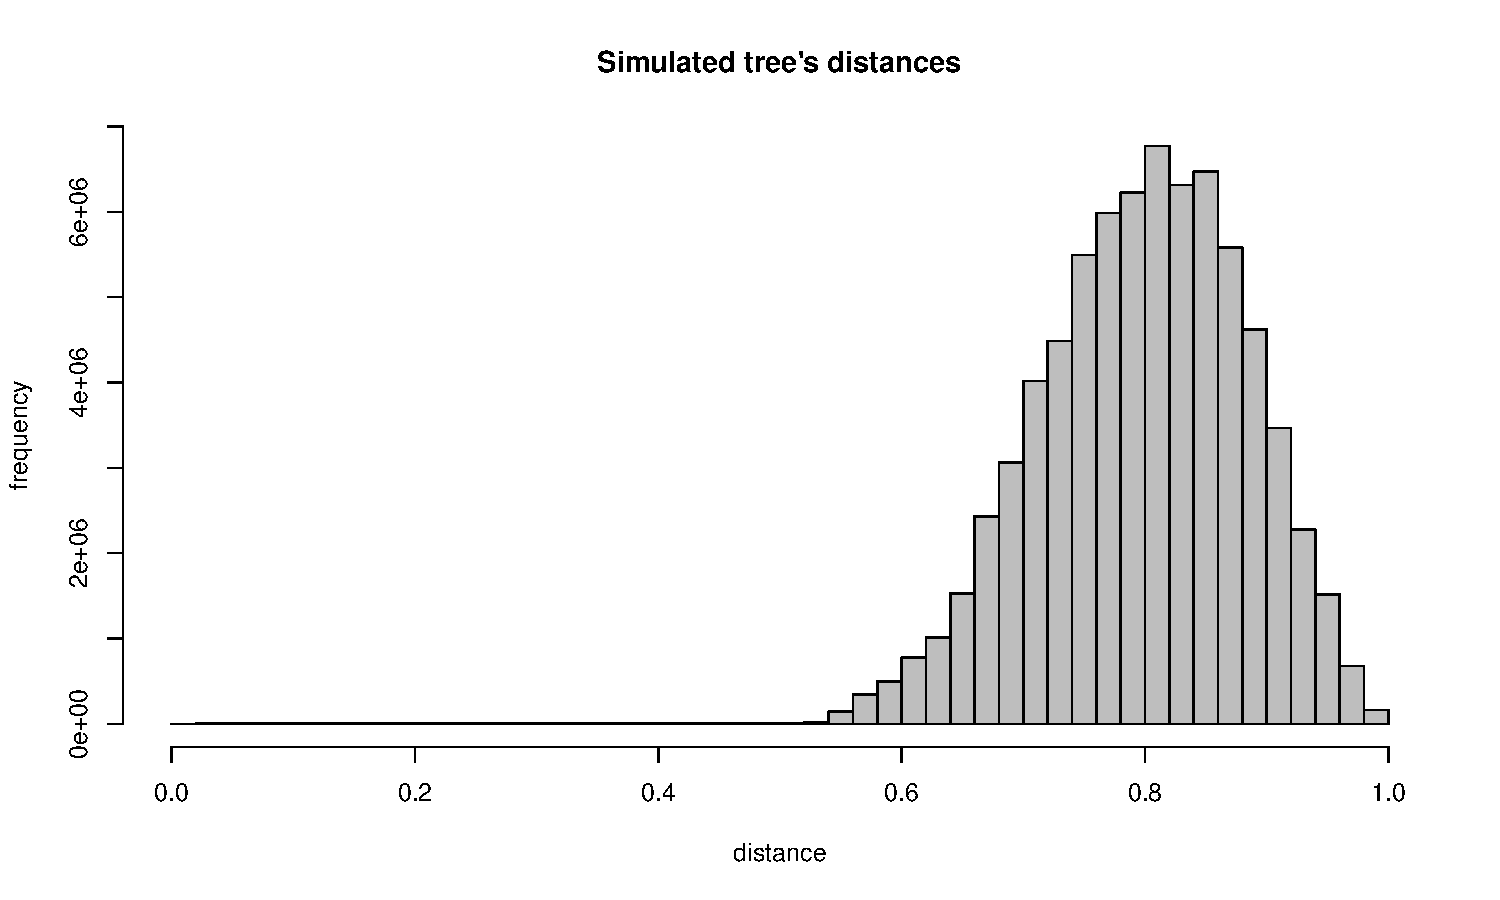
\includegraphics[width=10cm]{figure/plotget_distances-1} 
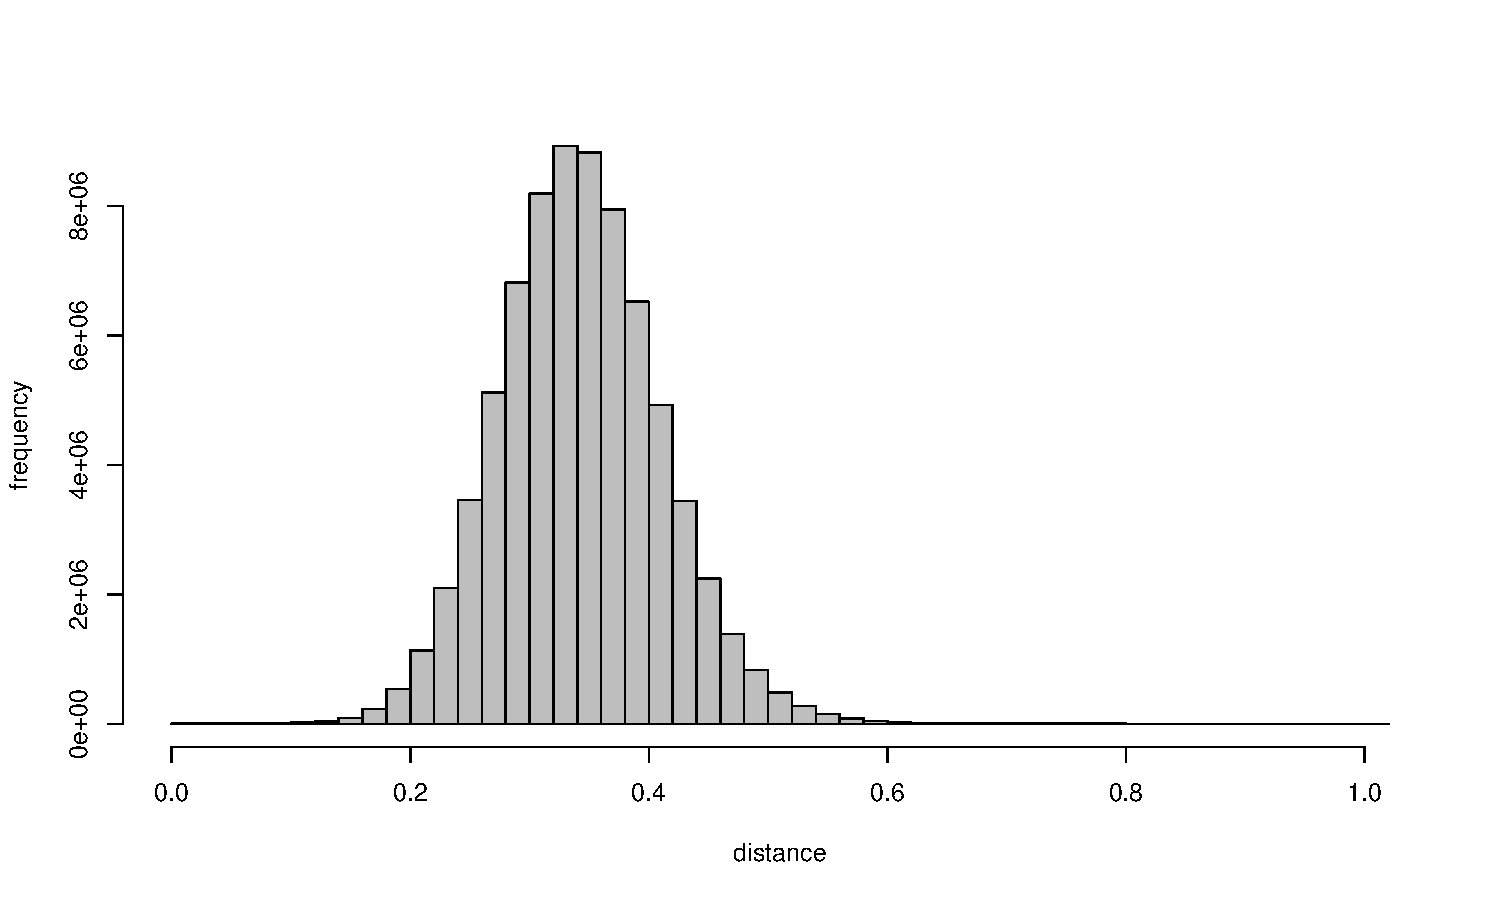
\includegraphics[width=10cm]{figure/plotget_distances-2} 

}



\end{knitrout}

\section{Clustering}
Clustering with fixed number of groups ?
\begin{knitrout}
\definecolor{shadecolor}{rgb}{0.969, 0.969, 0.969}\color{fgcolor}\begin{kframe}
\begin{alltt}
\hlstd{simhc} \hlkwb{<-} \hlkwd{hclust}\hlstd{(simx,} \hlkwc{method} \hlstd{=} \hlstr{"average"}\hlstd{)} \hlcom{# UPGMA}
\hlstd{ukhc} \hlkwb{<-} \hlkwd{hclust}\hlstd{(ukx,} \hlkwc{method} \hlstd{=} \hlstr{"average"}\hlstd{)}

\hlcom{##- cut based on height}
\hlkwa{if} \hlstd{(F)\{}
\hlcom{#- function of heights}
\hlstd{nheights} \hlkwb{<-} \hlnum{10} \hlcom{# number of threshold}
\hlstd{up} \hlkwb{<-} \hlkwd{round}\hlstd{(}\hlkwd{mean}\hlstd{(simx),} \hlnum{1}\hlstd{)} \hlcom{# cut up to the mean}
\hlcom{# breaks <-  seq(1/nbreaks, 1-(1/nbreaks), by = 1/nbreaks)}
\hlstd{simclus} \hlkwb{<-} \hlkwd{cutree}\hlstd{(simhc,} \hlkwc{h} \hlstd{=} \hlkwd{seq}\hlstd{(up} \hlopt{/} \hlstd{nheights, up,} \hlkwc{by} \hlstd{= up} \hlopt{/} \hlstd{nheights) )} \hlcom{# h = breaks}
\hlstd{up} \hlkwb{<-} \hlkwd{round}\hlstd{(}\hlkwd{mean}\hlstd{(ukx),}\hlnum{1}\hlstd{)} \hlcom{# cut up to the mean}
\hlstd{ukclus} \hlkwb{<-} \hlkwd{cutree}\hlstd{(ukhc,}  \hlkwc{h} \hlstd{=} \hlkwd{seq}\hlstd{(up} \hlopt{/} \hlstd{nheights, up,} \hlkwc{by} \hlstd{= up} \hlopt{/}\hlstd{nheights) )}
\hlcom{# rm(simx, ukx)}
\hlstd{\}}

\hlcom{#- cut as function of k groups}
\hlstd{kgroups} \hlkwb{<-} \hlkwd{c}\hlstd{(}\hlnum{500}\hlstd{,} \hlnum{1000}\hlstd{,} \hlnum{5000}\hlstd{,} \hlnum{8000}\hlstd{,} \hlnum{10000}\hlstd{)}
\hlstd{simclus} \hlkwb{<-} \hlkwd{cutree}\hlstd{(simhc,} \hlkwc{k} \hlstd{= kgroups )} \hlcom{# h = breaks}
\hlstd{ukclus} \hlkwb{<-} \hlkwd{cutree}\hlstd{(ukhc,}  \hlkwc{k} \hlstd{= kgroups )}
\hlcom{# colnames(simclus) <- paste("k",colnames(simclus),sep='')}
\hlcom{# colnames(ukclus) <- paste("k",colnames(ukclus),sep='')}
\hlkwd{head}\hlstd{(simclus)}
\end{alltt}
\begin{verbatim}
   500 1000 5000 8000 10000
7    1    1    1    1     1
8    2    2    2    2     2
9    3    3    3    3     3
10   4    4    4    4     4
11   5    5    5    5     5
12   6    6    6    6     6
\end{verbatim}
\begin{alltt}
\hlkwd{head}\hlstd{(ukclus)}
\end{alltt}
\begin{verbatim}
      500 1000 5000 8000 10000
34695   1    1    1    1     1
21677   1    1    1    1     1
72292   1    1    2    2     2
81292   1    1    1    3     3
85197   1    1    3    4     4
53538   1    1    4    5     5
\end{verbatim}
\begin{alltt}
\hlcom{##- Calculate size(=Freq) of each cluster across different threshold}
\hlstd{simfreqClust} \hlkwb{<-} \hlkwd{apply}\hlstd{(simclus,} \hlnum{2}\hlstd{,} \hlkwa{function}\hlstd{(}\hlkwc{x}\hlstd{)} \hlkwd{as.data.frame}\hlstd{(}\hlkwd{table}\hlstd{(x)))} \hlcom{# list}
\hlstd{ukfreqClust} \hlkwb{<-} \hlkwd{apply}\hlstd{(ukclus,} \hlnum{2}\hlstd{,} \hlkwa{function}\hlstd{(}\hlkwc{x}\hlstd{)} \hlkwd{as.data.frame}\hlstd{(}\hlkwd{table}\hlstd{(x)))}
\hlcom{# str(simfreqClust)}
\hlcom{# head(simfreqClust[[1]])}

\hlcom{##- number of different clusters by threshold # if number varies !}
\hlcom{# sapply(simfreqClust, function(x) dim(x)[1])}
\hlcom{# sapply(ukfreqClust, function(x) dim(x)[1])}

\hlcom{##- cluster size}
\hlcom{#- sim}
\hlkwd{sapply}\hlstd{(simfreqClust,} \hlkwa{function}\hlstd{(}\hlkwc{x}\hlstd{)} \hlkwd{summary}\hlstd{(x}\hlopt{$}\hlstd{Freq))}
\end{alltt}
\begin{verbatim}
            500    1000   5000  8000 10000
Min.       1.00    1.00  1.000  1.00 1.000
1st Qu.    2.00    2.00  1.000  1.00 1.000
Median     6.00    6.00  2.000  1.00 1.000
Mean      24.33   12.16  2.433  1.52 1.216
3rd Qu.   13.00   13.00  3.000  2.00 1.000
Max.    7395.00 3019.00 20.000 11.00 7.000
\end{verbatim}
\begin{alltt}
\hlcom{#- uk}
\hlkwd{sapply}\hlstd{(ukfreqClust,} \hlkwa{function}\hlstd{(}\hlkwc{x}\hlstd{)} \hlkwd{summary}\hlstd{(x}\hlopt{$}\hlstd{Freq))}
\end{alltt}
\begin{verbatim}
            500    1000    5000  8000  10000
Min.       1.00    1.00   1.000  1.00  1.000
1st Qu.    1.00    1.00   1.000  1.00  1.000
Median     2.00    2.00   1.000  1.00  1.000
Mean      24.33   12.16   2.433  1.52  1.216
3rd Qu.    7.00    6.00   2.000  1.00  1.000
Max.    6868.00 3486.00 142.000 86.00 39.000
\end{verbatim}
\begin{alltt}
\hlcom{##- percentiles}
\hlcom{# sapply(freqClust, function(x) round(quantile(x$Freq, }
\hlcom{# probs = c(0.01, 0.05, 0.1, 0.25, 0.5, 0.75, 0.95, 0.99, 1))))}
\hlcom{# }
\end{alltt}
\end{kframe}
\end{knitrout}

Distribution of sizes - semitransformed, transformed
\begin{knitrout}
\definecolor{shadecolor}{rgb}{0.969, 0.969, 0.969}\color{fgcolor}\begin{kframe}
\begin{alltt}
\hlcom{##- distr of cluster sizes: log(x) and Y untransformed}
\hlkwd{par}\hlstd{(}\hlkwc{mfcol}\hlstd{=}\hlkwd{c}\hlstd{(}\hlnum{2}\hlstd{,} \hlkwd{length}\hlstd{(kgroups)))}
\hlkwa{for} \hlstd{(i} \hlkwa{in} \hlnum{1}\hlopt{:}\hlkwd{length}\hlstd{(kgroups))\{}
  \hlstd{h} \hlkwb{<-} \hlkwd{hist}\hlstd{(}\hlkwd{log}\hlstd{(ukfreqClust[[i]]}\hlopt{$}\hlstd{Freq),}
       \hlkwc{main} \hlstd{=} \hlkwd{paste}\hlstd{(}\hlstr{"uk"}\hlstd{,} \hlkwd{names}\hlstd{(ukfreqClust)[i]),}
       \hlkwc{xlab} \hlstd{=} \hlstr{"log(size)"}\hlstd{)}
  \hlkwd{hist}\hlstd{(}\hlkwd{log}\hlstd{(simfreqClust[[i]]}\hlopt{$}\hlstd{Freq),}
       \hlkwc{main} \hlstd{=} \hlkwd{paste}\hlstd{(}\hlstr{"sim"}\hlstd{,} \hlkwd{names}\hlstd{(simfreqClust)[i]),}
       \hlkwc{xlab} \hlstd{=} \hlstr{"log(size)"}\hlstd{)}
\hlstd{\}}

\hlcom{##- distr of cluster sizes: log(x) and log(y)}
\hlkwd{par}\hlstd{(}\hlkwc{mfcol}\hlstd{=}\hlkwd{c}\hlstd{(}\hlnum{2}\hlstd{,} \hlkwd{length}\hlstd{(kgroups)))}
\hlkwa{for} \hlstd{(i} \hlkwa{in} \hlnum{1}\hlopt{:}\hlkwd{length}\hlstd{(kgroups))\{}
  \hlstd{h} \hlkwb{<-} \hlkwd{hist}\hlstd{(}\hlkwd{log}\hlstd{(ukfreqClust[[i]]}\hlopt{$}\hlstd{Freq),} \hlkwc{plot} \hlstd{= F)}
  \hlstd{h}\hlopt{$}\hlstd{counts} \hlkwb{<-} \hlkwd{log1p}\hlstd{(h}\hlopt{$}\hlstd{counts)} \hlcom{# log(y)}
  \hlkwd{plot}\hlstd{(h,} \hlkwc{ylab} \hlstd{=} \hlstr{"log(Freq)"}\hlstd{,}
       \hlkwc{main} \hlstd{=} \hlkwd{paste}\hlstd{(}\hlstr{"uk"}\hlstd{,} \hlkwd{names}\hlstd{(ukfreqClust)[i]),}
       \hlkwc{xlab} \hlstd{=} \hlstr{"log(size)"}\hlstd{)}

  \hlstd{h} \hlkwb{<-} \hlkwd{hist}\hlstd{(}\hlkwd{log}\hlstd{(simfreqClust[[i]]}\hlopt{$}\hlstd{Freq),} \hlkwc{plot} \hlstd{= F)}
  \hlstd{h}\hlopt{$}\hlstd{counts} \hlkwb{<-} \hlkwd{log1p}\hlstd{(h}\hlopt{$}\hlstd{counts)} \hlcom{# log(y)}
  \hlkwd{plot}\hlstd{(h,} \hlkwc{ylab} \hlstd{=} \hlstr{"log(Freq)"}\hlstd{,}
          \hlkwc{main} \hlstd{=} \hlkwd{paste}\hlstd{(}\hlstr{"sim"}\hlstd{,} \hlkwd{names}\hlstd{(simfreqClust)[i]),}
          \hlkwc{xlab} \hlstd{=} \hlstr{"log(size)"}\hlstd{)}

\hlstd{\}}
\end{alltt}
\end{kframe}

{\centering 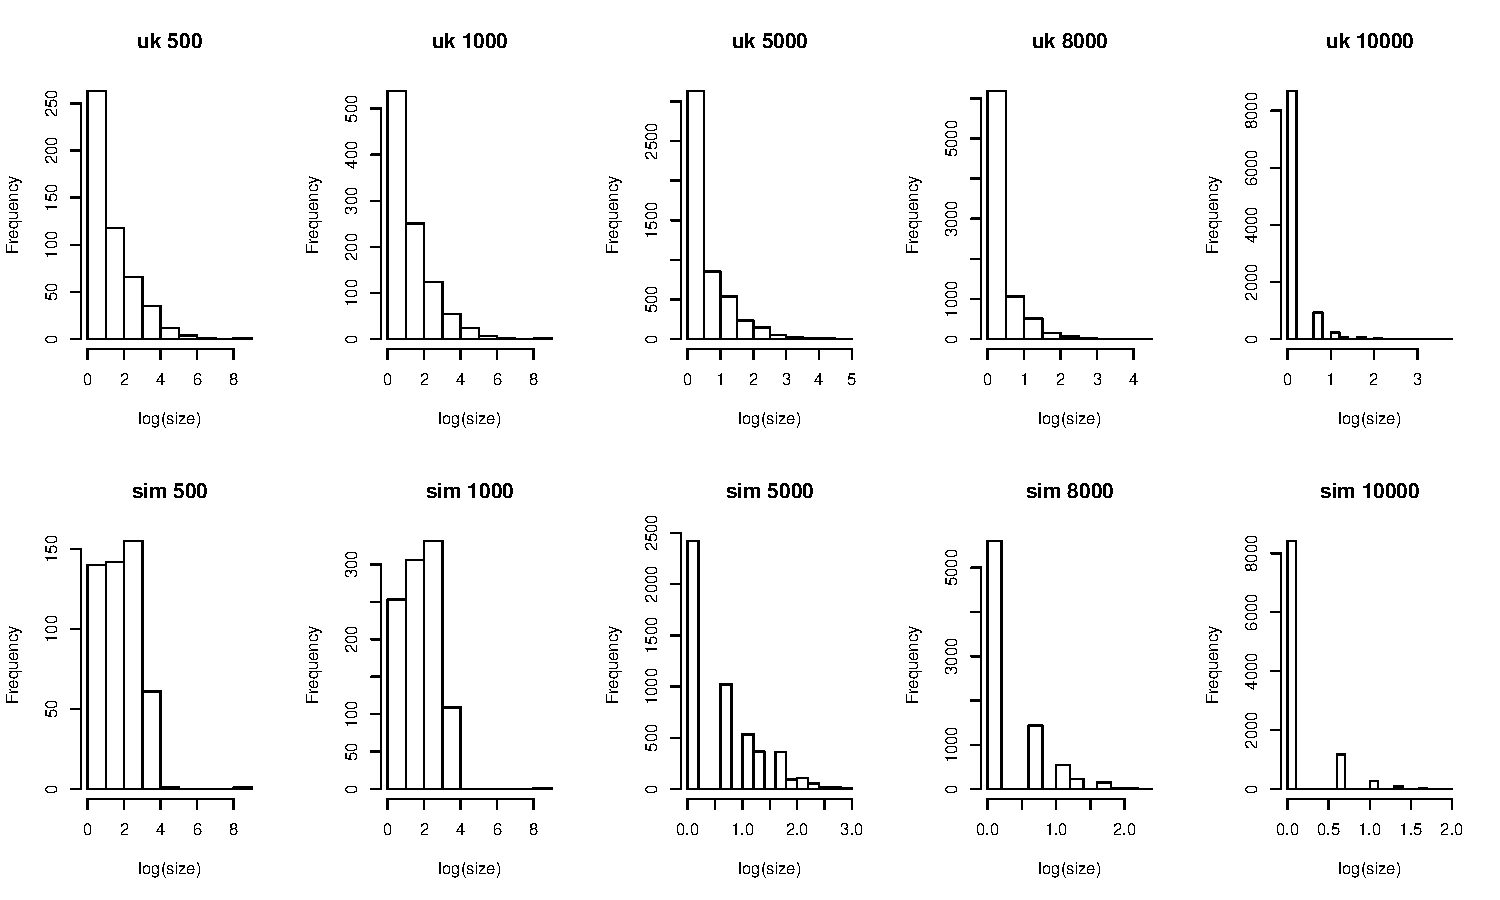
\includegraphics[width=10cm]{figure/plotplot_cluster_size-1} 
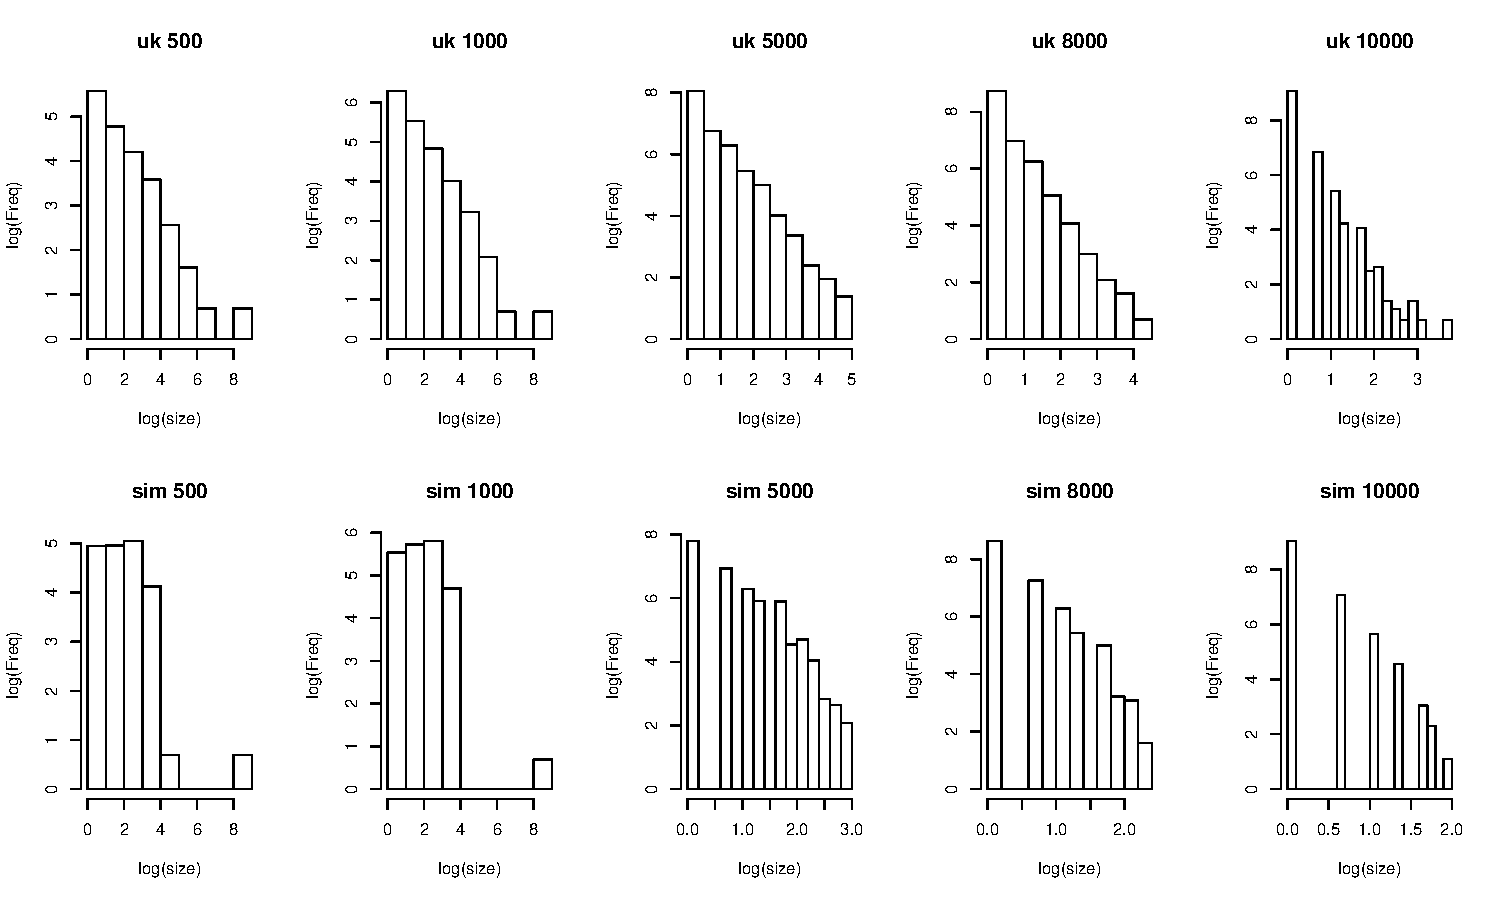
\includegraphics[width=10cm]{figure/plotplot_cluster_size-2} 

}



\end{knitrout}

QQ plot
\begin{knitrout}
\definecolor{shadecolor}{rgb}{0.969, 0.969, 0.969}\color{fgcolor}\begin{kframe}
\begin{alltt}
\hlkwd{par}\hlstd{(}\hlkwc{mfcol}\hlstd{=}\hlkwd{c}\hlstd{(}\hlnum{2}\hlstd{,} \hlkwd{length}\hlstd{(kgroups)))}
\hlkwa{for} \hlstd{(i} \hlkwa{in} \hlnum{1}\hlopt{:}\hlkwd{length}\hlstd{(kgroups))\{}
  \hlkwd{qqplot}\hlstd{(ukfreqClust[[i]]}\hlopt{$}\hlstd{Freq,}
         \hlstd{simfreqClust[[i]]}\hlopt{$}\hlstd{Freq,}
         \hlkwc{main} \hlstd{=} \hlkwd{names}\hlstd{(ukfreqClust)[i],}
         \hlkwc{xlab} \hlstd{=} \hlstr{"uk"}\hlstd{,} \hlkwc{ylab} \hlstd{=} \hlstr{"sim"}\hlstd{)}

  \hlkwd{qqplot}\hlstd{(}\hlkwd{log}\hlstd{(ukfreqClust[[i]]}\hlopt{$}\hlstd{Freq),}
         \hlkwd{log}\hlstd{(simfreqClust[[i]]}\hlopt{$}\hlstd{Freq),}
         \hlkwc{main} \hlstd{=} \hlkwd{names}\hlstd{(ukfreqClust)[i],}
         \hlkwc{xlab} \hlstd{=} \hlstr{"log(uk)"}\hlstd{,} \hlkwc{ylab} \hlstd{=} \hlstr{"log(sim)"}\hlstd{)}

\hlstd{\}}
\end{alltt}
\end{kframe}

{\centering 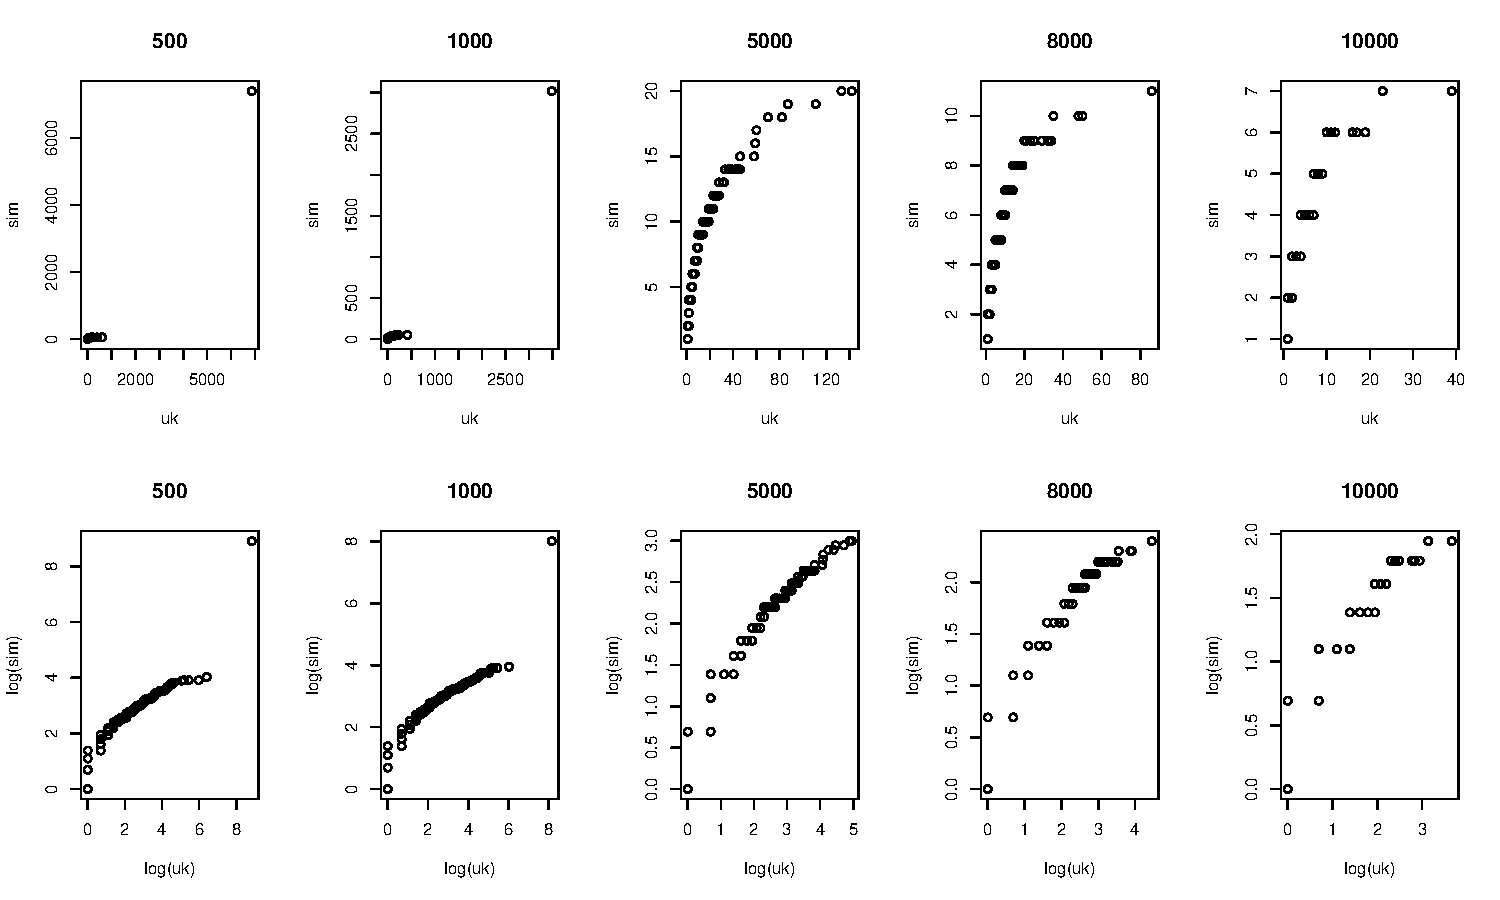
\includegraphics[width=10cm]{figure/plotQQ_plot-1} 

}



\end{knitrout}
% ggplot unecessary

\section{Add patients data}
Add data from sample states and time
\begin{knitrout}
\definecolor{shadecolor}{rgb}{0.969, 0.969, 0.969}\color{fgcolor}\begin{kframe}
\begin{alltt}
\hlcom{##- converting sample states in table of co-variates ?}
\hlstd{demes} \hlkwb{<-} \hlkwd{as.vector}\hlstd{(}\hlkwd{read.csv}\hlstd{(}\hlkwc{file} \hlstd{=} \hlstr{"demes.csv"}\hlstd{)}\hlopt{$}\hlstd{x)}
\hlstd{sampleTimes} \hlkwb{<-} \hlkwd{scan}\hlstd{(} \hlkwc{file} \hlstd{=} \hlstr{'sampleTimes'} \hlstd{)}
\hlstd{ss}  \hlkwb{<-} \hlkwd{matrix}\hlstd{(} \hlkwd{scan}\hlstd{(} \hlkwc{file} \hlstd{=} \hlstr{'sampleStates'} \hlstd{) ,}
               \hlkwc{byrow} \hlstd{=} \hlnum{TRUE}\hlstd{,}
               \hlkwc{ncol} \hlstd{=} \hlkwd{length}\hlstd{(demes))}
\hlkwd{colnames}\hlstd{(ss)} \hlkwb{<-} \hlstd{demes}
\hlkwd{dim}\hlstd{(ss)}
\end{alltt}
\begin{verbatim}
[1] 12164   121
\end{verbatim}
\begin{alltt}
\hlkwd{max}\hlstd{(ss[,}\hlnum{121}\hlstd{])} \hlcom{# nothing on source}
\end{alltt}
\begin{verbatim}
[1] 0
\end{verbatim}
\begin{alltt}
\hlstd{demo} \hlkwb{<-} \hlkwd{data.frame}\hlstd{()}
\hlkwa{for} \hlstd{(i} \hlkwa{in} \hlnum{1}\hlopt{:}\hlkwd{dim}\hlstd{(ss)[}\hlnum{1}\hlstd{])\{} \hlcom{# dim(ss)[1]}
  \hlstd{deme} \hlkwb{<-} \hlkwd{names}\hlstd{(}\hlkwd{which}\hlstd{(ss[i,]} \hlopt{==} \hlnum{1}\hlstd{))} \hlcom{# name of column which has value 1}
  \hlstd{patient} \hlkwb{<-} \hlstd{i}
  \hlstd{time} \hlkwb{<-} \hlstd{sampleTimes[i]}
  \hlstd{age} \hlkwb{<-} \hlkwd{as.numeric}\hlstd{(} \hlkwd{regmatches}\hlstd{( deme,}
                \hlkwd{regexec}\hlstd{(} \hlstr{"\textbackslash{}\textbackslash{}.age([0-9])"}\hlstd{, deme) )[[}\hlnum{1}\hlstd{]][}\hlnum{2}\hlstd{] )}
  \hlstd{care} \hlkwb{<-} \hlkwd{as.numeric}\hlstd{(} \hlkwd{regmatches}\hlstd{( deme,}
                \hlkwd{regexec}\hlstd{(} \hlstr{"care([0-9])"}\hlstd{, deme) )[[}\hlnum{1}\hlstd{]][}\hlnum{2}\hlstd{] )}
  \hlstd{stage} \hlkwb{<-} \hlkwd{as.numeric}\hlstd{(} \hlkwd{regmatches}\hlstd{( deme,}
                \hlkwd{regexec}\hlstd{(} \hlstr{"stage([0-9])"}\hlstd{, deme) )[[}\hlnum{1}\hlstd{]][}\hlnum{2}\hlstd{] )}
  \hlstd{risk} \hlkwb{<-} \hlkwd{as.numeric}\hlstd{(} \hlkwd{regmatches}\hlstd{( deme,}
                \hlkwd{regexec}\hlstd{(} \hlstr{"riskLevel([0-9])"}\hlstd{, deme) )[[}\hlnum{1}\hlstd{]][}\hlnum{2}\hlstd{] )}
  \hlstd{demo} \hlkwb{<-} \hlkwd{rbind}\hlstd{(demo,} \hlkwd{cbind}\hlstd{(}
    \hlstd{patient, time, age, care, stage, risk))}
\hlstd{\}}
\hlkwd{str}\hlstd{(demo)}
\end{alltt}
\begin{verbatim}
'data.frame':	12164 obs. of  6 variables:
 $ patient: num  1 2 3 4 5 6 7 8 9 10 ...
 $ time   : num  11245 8627 6679 8446 8900 ...
 $ age    : num  3 3 4 4 4 3 4 3 3 4 ...
 $ care   : num  1 1 1 1 1 1 1 1 1 1 ...
 $ stage  : num  1 1 1 5 4 2 5 2 3 5 ...
 $ risk   : num  1 1 1 1 1 1 1 1 2 1 ...
\end{verbatim}
\begin{alltt}
\hlcom{##- date of diagnosis ?}
\hlstd{date0} \hlkwb{<-} \hlkwd{as.Date}\hlstd{(}\hlstr{'1979-01-01'}\hlstd{)}
\hlstd{demo}\hlopt{$}\hlstd{datediag} \hlkwb{<-} \hlstd{date0} \hlopt{+} \hlstd{demo}\hlopt{$}\hlstd{time}
\hlkwd{min}\hlstd{(demo}\hlopt{$}\hlstd{datediag)}
\end{alltt}
\begin{verbatim}
[1] "1996-11-15"
\end{verbatim}
\begin{alltt}
\hlkwd{max}\hlstd{(demo}\hlopt{$}\hlstd{datediag)}
\end{alltt}
\begin{verbatim}
[1] "2013-02-15"
\end{verbatim}
\end{kframe}
\end{knitrout}

Add cluster size by patient
\begin{knitrout}
\definecolor{shadecolor}{rgb}{0.969, 0.969, 0.969}\color{fgcolor}\begin{kframe}
\begin{alltt}
\hlcom{##- function to calculate both numclus and sizeclus for each seqindex into a LIST}
\hlcom{##- with same variable names}
  \hlcom{##- in list}
  \hlstd{l} \hlkwb{<-} \hlkwd{list}\hlstd{()}
  \hlkwa{for} \hlstd{(i} \hlkwa{in} \hlnum{1}\hlopt{:}\hlkwd{length}\hlstd{(kgroups)) \{}

  \hlcom{#- cluster number}
  \hlstd{numclus} \hlkwb{<-} \hlkwd{as.data.frame}\hlstd{(simclus[, i])}
  \hlstd{numclus} \hlkwb{<-} \hlkwd{cbind}\hlstd{(}\hlkwd{rownames}\hlstd{(numclus), numclus)}
  \hlkwd{colnames}\hlstd{(numclus)} \hlkwb{<-} \hlkwd{c}\hlstd{(}\hlstr{"id"}\hlstd{,} \hlstr{"num"}\hlstd{)}
  \hlkwd{row.names}\hlstd{(numclus)} \hlkwb{<-} \hlkwa{NULL}
  \hlcom{# head(numclus)}

  \hlcom{#- size of cluster}
  \hlstd{a} \hlkwb{<-} \hlkwd{merge}\hlstd{(}\hlkwc{x} \hlstd{= numclus,} \hlkwc{y} \hlstd{= simfreqClust[[i]],}
             \hlkwc{by.x} \hlstd{=} \hlstr{"num"}\hlstd{,} \hlkwc{by.y} \hlstd{=} \hlstr{"x"}\hlstd{,}
             \hlkwc{all.x} \hlstd{=} \hlnum{TRUE}\hlstd{,} \hlkwc{sort} \hlstd{=} \hlnum{FALSE}\hlstd{)}
  \hlcom{#- binary clustering variable}
  \hlstd{a}\hlopt{$}\hlstd{Clus} \hlkwb{<-} \hlkwd{ifelse}\hlstd{(a}\hlopt{$}\hlstd{Freq} \hlopt{>} \hlnum{1}\hlstd{,} \hlnum{1}\hlstd{,} \hlnum{0}\hlstd{)}
  \hlcom{#- colnames}
  \hlkwd{colnames}\hlstd{(a)[}\hlkwd{which}\hlstd{(}\hlkwd{colnames}\hlstd{(a)} \hlopt{==}\hlstr{"Freq"}\hlstd{)]} \hlkwb{<-} \hlstr{"size"}
  \hlkwd{colnames}\hlstd{(a)[}\hlkwd{which}\hlstd{(}\hlkwd{colnames}\hlstd{(a)} \hlopt{==}\hlstr{"Clus"}\hlstd{)]} \hlkwb{<-} \hlstr{"clus"}
  \hlstd{l[[i]]} \hlkwb{<-} \hlstd{a}
  \hlkwd{names}\hlstd{(l)[i]} \hlkwb{<-} \hlkwd{names}\hlstd{(simfreqClust[i])}
  \hlstd{\}}

  \hlkwd{rm}\hlstd{(a, numclus)}
\hlcom{# str(l)}

\hlcom{##-proportion in or out clusters}
\hlkwd{sapply}\hlstd{(l,} \hlkwa{function}\hlstd{(}\hlkwc{x}\hlstd{)} \hlkwd{round}\hlstd{(}\hlkwd{prop.table}\hlstd{(}\hlkwd{table}\hlstd{(x}\hlopt{$}\hlstd{clus)),}\hlnum{2}\hlstd{))}
\end{alltt}
\begin{verbatim}
   500 1000 5000 8000 10000
0 0.01 0.01  0.2 0.46  0.69
1 0.99 0.99  0.8 0.54  0.31
\end{verbatim}
\begin{alltt}
\hlcom{##- cluster sizes}
\hlkwd{sapply}\hlstd{(l,} \hlkwa{function}\hlstd{(}\hlkwc{x}\hlstd{)} \hlkwd{summary}\hlstd{(x}\hlopt{$}\hlstd{size))}
\end{alltt}
\begin{verbatim}
         500   1000   5000   8000 10000
Min.       1    1.0  1.000  1.000 1.000
1st Qu.   22   11.0  2.000  1.000 1.000
Median  7395   21.0  4.000  2.000 1.000
Mean    4504  762.7  4.425  2.223 1.488
3rd Qu. 7395   52.0  6.000  3.000 2.000
Max.    7395 3019.0 20.000 11.000 7.000
\end{verbatim}
\end{kframe}
\end{knitrout}

\begin{knitrout}
\definecolor{shadecolor}{rgb}{0.969, 0.969, 0.969}\color{fgcolor}\begin{kframe}
\begin{alltt}
\hlstd{listclus} \hlkwb{<-} \hlkwd{lapply}\hlstd{(l,} \hlkwa{function}\hlstd{(}\hlkwc{x}\hlstd{)}
\hlkwd{merge}\hlstd{(x, demo,}
      \hlkwc{by.x} \hlstd{=} \hlstr{"id"}\hlstd{,} \hlkwc{by.y} \hlstd{=} \hlstr{"patient"}\hlstd{,}
      \hlkwc{all.x} \hlstd{= T,} \hlkwc{sort} \hlstd{=} \hlnum{FALSE}\hlstd{))}

\hlcom{# head(listclus[[4]])}
\hlcom{# table(listclus[[4]]$clus)}
\end{alltt}
\end{kframe}
\end{knitrout}

\section{Regressions}

\subsection{Logistic}
\begin{knitrout}
\definecolor{shadecolor}{rgb}{0.969, 0.969, 0.969}\color{fgcolor}\begin{kframe}
\begin{alltt}
\hlcom{##- model: clus ~ age +  stage + time + risk}
\hlcom{##- care = 1 for all at diagnosis}
\hlcom{## ex. }
\hlstd{logit_model} \hlkwb{=} \hlstr{"clus ~ age + stage + time + risk"}
\hlstd{logit_model_std} \hlkwb{=} \hlstr{"clus ~ scale(age) + scale(stage) + scale(time) + scale(risk)"}
\hlopt{?}\hlstd{glm}
\hlkwd{lapply}\hlstd{(listclus,} \hlkwa{function}\hlstd{(}\hlkwc{x}\hlstd{)} \hlkwd{summary}\hlstd{(}\hlkwd{glm}\hlstd{(}\hlkwc{formula} \hlstd{= logit_model_std,}
                                 \hlkwc{data} \hlstd{= x,}
                                 \hlkwc{family} \hlstd{=} \hlkwd{binomial}\hlstd{(}\hlkwc{link} \hlstd{=} \hlstr{"logit"}\hlstd{))))}
\end{alltt}
\begin{verbatim}
$`500`

Call:
glm(formula = logit_model_std, family = binomial(link = "logit"), 
    data = x)

Deviance Residuals: 
    Min       1Q   Median       3Q      Max  
-3.2932   0.1035   0.1089   0.1179   0.1598  

Coefficients:
             Estimate Std. Error z value Pr(>|z|)    
(Intercept)   5.06851    0.11629  43.585   <2e-16 ***
scale(age)    0.07370    0.11120   0.663   0.5075    
scale(stage)  0.01809    0.11472   0.158   0.8747    
scale(time)  -0.09012    0.11632  -0.775   0.4385    
scale(risk)  -0.18421    0.10107  -1.823   0.0684 .  
---
Signif. codes:  0 '***' 0.001 '**' 0.01 '*' 0.05 '.' 0.1 ' ' 1

(Dispersion parameter for binomial family taken to be 1)

    Null deviance: 943.23  on 12163  degrees of freedom
Residual deviance: 939.00  on 12159  degrees of freedom
AIC: 949

Number of Fisher Scoring iterations: 8


$`1000`

Call:
glm(formula = logit_model_std, family = binomial(link = "logit"), 
    data = x)

Deviance Residuals: 
    Min       1Q   Median       3Q      Max  
-3.2188   0.1310   0.1442   0.1589   0.2238  

Coefficients:
             Estimate Std. Error z value Pr(>|z|)    
(Intercept)   4.55488    0.09111  49.994   <2e-16 ***
scale(age)    0.05994    0.08537   0.702   0.4826    
scale(stage)  0.02410    0.08834   0.273   0.7850    
scale(time)  -0.22805    0.09289  -2.455   0.0141 *  
scale(risk)  -0.16634    0.07873  -2.113   0.0346 *  
---
Signif. codes:  0 '***' 0.001 '**' 0.01 '*' 0.05 '.' 0.1 ' ' 1

(Dispersion parameter for binomial family taken to be 1)

    Null deviance: 1456.7  on 12163  degrees of freedom
Residual deviance: 1445.4  on 12159  degrees of freedom
AIC: 1455.4

Number of Fisher Scoring iterations: 7


$`5000`

Call:
glm(formula = logit_model_std, family = binomial(link = "logit"), 
    data = x)

Deviance Residuals: 
    Min       1Q   Median       3Q      Max  
-1.8353   0.6524   0.6639   0.6708   0.6828  

Coefficients:
              Estimate Std. Error z value Pr(>|z|)    
(Intercept)   1.393642   0.022721  61.338   <2e-16 ***
scale(age)    0.001913   0.022860   0.084    0.933    
scale(stage)  0.002938   0.022910   0.128    0.898    
scale(time)  -0.024301   0.022878  -1.062    0.288    
scale(risk)   0.013449   0.022864   0.588    0.556    
---
Signif. codes:  0 '***' 0.001 '**' 0.01 '*' 0.05 '.' 0.1 ' ' 1

(Dispersion parameter for binomial family taken to be 1)

    Null deviance: 12135  on 12163  degrees of freedom
Residual deviance: 12134  on 12159  degrees of freedom
AIC: 12144

Number of Fisher Scoring iterations: 4


$`8000`

Call:
glm(formula = logit_model_std, family = binomial(link = "logit"), 
    data = x)

Deviance Residuals: 
   Min      1Q  Median      3Q     Max  
-1.265  -1.245   1.095   1.111   1.142  

Coefficients:
               Estimate Std. Error z value Pr(>|z|)    
(Intercept)   0.1585314  0.0181926   8.714   <2e-16 ***
scale(age)   -0.0006118  0.0183335  -0.033    0.973    
scale(stage)  0.0180774  0.0183458   0.985    0.324    
scale(time)  -0.0027158  0.0182654  -0.149    0.882    
scale(risk)  -0.0204569  0.0181770  -1.125    0.260    
---
Signif. codes:  0 '***' 0.001 '**' 0.01 '*' 0.05 '.' 0.1 ' ' 1

(Dispersion parameter for binomial family taken to be 1)

    Null deviance: 16787  on 12163  degrees of freedom
Residual deviance: 16784  on 12159  degrees of freedom
AIC: 16794

Number of Fisher Scoring iterations: 3


$`10000`

Call:
glm(formula = logit_model_std, family = binomial(link = "logit"), 
    data = x)

Deviance Residuals: 
    Min       1Q   Median       3Q      Max  
-0.9038  -0.8656  -0.8471   1.5116   1.6187  

Coefficients:
             Estimate Std. Error z value Pr(>|z|)    
(Intercept)  -0.80789    0.01964 -41.132   <2e-16 ***
scale(age)    0.02309    0.01985   1.163    0.245    
scale(stage)  0.03683    0.01981   1.859    0.063 .  
scale(time)   0.02224    0.01975   1.126    0.260    
scale(risk)  -0.01789    0.01974  -0.906    0.365    
---
Signif. codes:  0 '***' 0.001 '**' 0.01 '*' 0.05 '.' 0.1 ' ' 1

(Dispersion parameter for binomial family taken to be 1)

    Null deviance: 15031  on 12163  degrees of freedom
Residual deviance: 15024  on 12159  degrees of freedom
AIC: 15034

Number of Fisher Scoring iterations: 4
\end{verbatim}
\begin{alltt}
\hlcom{# logistic <- function(x, m = logit_model)\{}
\hlcom{#   fit <- glm(m , data = x, }
\hlcom{#                    family = binomial(link = "logit"))}
\hlcom{#   co <- coef(summary(fit))}
\hlcom{#   ## odds ratios and 95% CI}
\hlcom{#   # or <- exp(cbind(OR = coef(fit), confint(fit)))}
\hlcom{#   # return(list(co, or))}
\hlcom{#   return(cbind(co[,c(1,4)]))}
\hlcom{# \}}
\hlcom{# }
\hlcom{# ##- test 1 level}
\hlcom{# c <- listclus[[1]]}
\hlcom{# logistic(x = c, m = logit_model_std)}
\hlcom{# }
\hlcom{# ##- all levels}
\hlcom{# lapply(listclus, function(x) logistic(x, m = logit_model_std))}
\end{alltt}
\end{kframe}
\end{knitrout}

\subsection{Linear}
\begin{knitrout}
\definecolor{shadecolor}{rgb}{0.969, 0.969, 0.969}\color{fgcolor}\begin{kframe}
\begin{alltt}
\hlstd{lm_model} \hlkwb{=} \hlstr{"size ~ age + stage + time + risk"}
\hlstd{lm_model_std} \hlkwb{=} \hlstr{"scale(size) ~ scale(age) + scale(stage) + scale(time) + scale(risk)"}

\hlkwd{lapply}\hlstd{(listclus,} \hlkwa{function}\hlstd{(}\hlkwc{x}\hlstd{)} \hlkwd{summary}\hlstd{(}\hlkwd{lm}\hlstd{(lm_model_std,} \hlkwc{data} \hlstd{= x)))}
\end{alltt}
\begin{verbatim}
$`500`

Call:
lm(formula = lm_model_std, data = x)

Residuals:
    Min      1Q  Median      3Q     Max 
-1.2705 -1.2414  0.7943  0.8052  0.8286 

Coefficients:
               Estimate Std. Error t value Pr(>|t|)
(Intercept)  -2.824e-14  9.068e-03   0.000    1.000
scale(age)   -4.245e-04  9.139e-03  -0.046    0.963
scale(stage) -6.856e-03  9.144e-03  -0.750    0.453
scale(time)   4.858e-03  9.104e-03   0.534    0.594
scale(risk)  -2.027e-03  9.070e-03  -0.224    0.823

Residual standard error: 1 on 12159 degrees of freedom
Multiple R-squared:  8.078e-05,	Adjusted R-squared:  -0.0002482 
F-statistic: 0.2456 on 4 and 12159 DF,  p-value: 0.9125


$`1000`

Call:
lm(formula = lm_model_std, data = x)

Residuals:
    Min      1Q  Median      3Q     Max 
-0.6277 -0.5808 -0.5659 -0.5336  1.7610 

Coefficients:
               Estimate Std. Error t value Pr(>|t|)
(Intercept)  -2.208e-14  9.067e-03   0.000    1.000
scale(age)   -1.427e-02  9.138e-03  -1.562    0.118
scale(stage) -1.947e-03  9.144e-03  -0.213    0.831
scale(time)   1.686e-03  9.103e-03   0.185    0.853
scale(risk)   1.506e-03  9.070e-03   0.166    0.868

Residual standard error: 1 on 12159 degrees of freedom
Multiple R-squared:  0.0002211,	Adjusted R-squared:  -0.0001078 
F-statistic: 0.6724 on 4 and 12159 DF,  p-value: 0.6111


$`5000`

Call:
lm(formula = lm_model_std, data = x)

Residuals:
    Min      1Q  Median      3Q     Max 
-1.0397 -0.6975 -0.1676  0.4660  4.5356 

Coefficients:
               Estimate Std. Error t value Pr(>|t|)  
(Intercept)   2.744e-16  9.067e-03   0.000   1.0000  
scale(age)    8.351e-04  9.137e-03   0.091   0.9272  
scale(stage) -2.079e-04  9.143e-03  -0.023   0.9819  
scale(time)   3.411e-03  9.103e-03   0.375   0.7079  
scale(risk)   1.969e-02  9.069e-03   2.171   0.0299 *
---
Signif. codes:  0 '***' 0.001 '**' 0.01 '*' 0.05 '.' 0.1 ' ' 1

Residual standard error: 1 on 12159 degrees of freedom
Multiple R-squared:  0.0004,	Adjusted R-squared:  7.114e-05 
F-statistic: 1.216 on 4 and 12159 DF,  p-value: 0.3015


$`8000`

Call:
lm(formula = lm_model_std, data = x)

Residuals:
    Min      1Q  Median      3Q     Max 
-0.7774 -0.7385 -0.1467  0.4663  5.3336 

Coefficients:
               Estimate Std. Error t value Pr(>|t|)
(Intercept)   2.257e-15  9.068e-03   0.000    1.000
scale(age)   -5.272e-03  9.138e-03  -0.577    0.564
scale(stage)  8.204e-03  9.144e-03   0.897    0.370
scale(time)   7.313e-03  9.104e-03   0.803    0.422
scale(risk)  -1.942e-03  9.070e-03  -0.214    0.830

Residual standard error: 1 on 12159 degrees of freedom
Multiple R-squared:  0.000139,	Adjusted R-squared:  -0.0001899 
F-statistic: 0.4227 on 4 and 12159 DF,  p-value: 0.7924


$`10000`

Call:
lm(formula = lm_model_std, data = x)

Residuals:
    Min      1Q  Median      3Q     Max 
-0.6097 -0.5563 -0.5292  0.5587  6.2095 

Coefficients:
               Estimate Std. Error t value Pr(>|t|)  
(Intercept)  -1.373e-15  9.065e-03   0.000   1.0000  
scale(age)    9.973e-03  9.136e-03   1.092   0.2750  
scale(stage)  2.187e-02  9.142e-03   2.392   0.0168 *
scale(time)   9.734e-03  9.101e-03   1.070   0.2848  
scale(risk)   2.170e-03  9.067e-03   0.239   0.8109  
---
Signif. codes:  0 '***' 0.001 '**' 0.01 '*' 0.05 '.' 0.1 ' ' 1

Residual standard error: 0.9998 on 12159 degrees of freedom
Multiple R-squared:  0.0006847,	Adjusted R-squared:  0.000356 
F-statistic: 2.083 on 4 and 12159 DF,  p-value: 0.08024
\end{verbatim}
\end{kframe}
\end{knitrout}





\end{document}
